%% ---------------------------------------------------------------------
%% Electronic supplementary material.
%%
%% This file holds material referenced from the article but carried outside
%% its page count. It is deliberately self-contained: it repeats enough of
%% each quantity's definition that a reader arriving here from the article
%% does not have to hold the article open beside it.
%%
%% Build: pdflatex supplementary
%% ---------------------------------------------------------------------
\documentclass[11pt]{article}
\usepackage[margin=1in]{geometry}
\usepackage{booktabs}
\usepackage{amsmath}
\usepackage{graphicx}
%% CROSS-DOCUMENT REFERENCES. Article table numbers were hardcoded here and two
%% of the three were already wrong. xr resolves \ref against the article's own
%% labels via main.aux, so an inserted table cannot silently invalidate them.
%% Build the article first; that is the order the submission check uses.
\usepackage{xr}
\externaldocument{main}
%% Same semantic style for the law's readout term as the article defines.
\newcommand{\readout}{\textit{readout}}

\title{Supplementary material\\
\large When does fusing hand-crafted knowledge with learned representations
pay? A cost-normalized benchmark of stacking, substitution and interference}
\date{}

\begin{document}
\maketitle

\section*{S1. The self-supervised margin, at every measured fraction}

The prior's own gain envelopes are in the article (Tables~\ref{tab:envelope},
\ref{tab:domainenv} and \ref{tab:vitenvelope}). This
table gives the remaining envelope those tables summarize in prose: the margin
of a $2\times$-compute SimCLR initialization over the $1.02\times$ prior on
CIFAR-100 with ResNet-18, under plain crop-and-flip augmentation, at every
measured data fraction. Every entry is a paired difference against a shared
baseline arm under the article's frozen recipe, so a positive entry is a
fraction where the $2\times$-compute initialization wins.

The shape is the point: the margin is unimodal. The self-supervised
advantage is a mid-band phenomenon that starves below $1$--$2\%$, where too
few images are available to contrast, and decays to nothing by $50\%$, where
the data itself dominates and every intervention converges.

\begin{table}[htbp]
\centering
\caption{SimCLR initialization ($2\times$ compute) minus the prior
($1.02\times$), CIFAR-100 / ResNet-18, plain augmentation. Three seeds per
cell. At $5\times$ pre-training compute the margin instead runs $+3.1$ to
$+9.2$ over $1$--$15\%$, narrowing to $+2.6$ at $25\%$ (article,
Sec.~\ref{sec:budget}).}
\label{tab:appssl}
\begin{tabular}{lrlr}
\toprule
Frac. & SSL $-$ prior & Frac. & SSL $-$ prior \\
\midrule
1\% & $+0.85$ & 10\%  & $+5.01$ \\
2\% & $+2.38$ & 15\%  & $+4.09$ \\
3\% & $+2.31$ & 50\%  & $+0.73$ \\
5\% & $+3.90$ & 100\% & $+0.22$ \\
7\% & $+4.99$ &       & \\
\bottomrule
\end{tabular}
\end{table}

\section*{S2. The law's components}

The article states the decomposition $\Delta = G + \readout$ and audits
the sign of its second term. The component curves behind that audit are
collected here.

\paragraph{Feature-gain curves.} $G$ is non-monotone in data and
dataset-specific in shape: CIFAR-10 $4.81$, $5.52$, $3.97$, $0.65$ at $0.5$,
$1$, $2.5$, $5$k images; CIFAR-100 $4.16$, $5.14$, $6.26$, $3.55$;
Tiny-ImageNet falls monotonically $4.19$, $2.66$, $1.70$ ($1$, $5$, $10$k);
STL-10 $4.70$, $4.97$, $3.20$. Where the \readout{} term is flat, the envelope
peak coincides with the $G$ peak: the envelope's shape \emph{is} the
feature-gain curve.

\paragraph{The \readout{} branch.} Mapped on ceiling-free CIFAR-10: $+1.56$ at
baseline $39.2$, $+1.14$ at $51.7$ and $+0.44$ at both $69.1$ and $80.7$,
positive throughout and decaying toward sufficiency. Below the crossing it
reaches $-2.7$ at bases $8.9$ and $5.3$. The bracket $[31.8, 40.3]$ used
throughout the article is pinned by a Swin cell still negative at $31.8$ and a
convolutional cell already positive at $40.3$.

\paragraph{Label-space crossings.} On byte-identical CIFAR-100 pixels, a full
$2{\times}2$ of training against evaluation label space (100-way vs.\ 20-way)
moves $G$ by at most $1\sigma$. On Tiny-ImageNet the same crossing finds two
real opposing effects (evaluation-space $+1.9$, checkpoint-set $+1.6$, both
${\sim}5\sigma$) that cancel on the diagonal, which is why $G$ comparisons in
the article always fix the evaluation space.

\section*{S3. An illustrative panel, and why it is not evidence}

The measurements behind the prior's feature effect are the alignment statistic
and the linear evaluation of the article's Sec.~\ref{sec:imprint}. The panel below only
illustrates them, and is reproduced precisely because it shows the effect
\emph{less} clearly than the numbers do.

\begin{figure}[htbp]
\centering

\includegraphics[width=0.62\linewidth]{figs_explain/tsne_auxmag_5pct_sched0.png}
\caption{t-SNE of frozen penultimate test features, first eight classes,
baseline (top) and prior arm (bottom), CIFAR-100 at 5\%. The silhouette in
each title is computed over \emph{all} classes in the \emph{full} feature
space and moves only from $-0.072$ to $-0.064$: this projection does
\emph{not} show the $+6.3$-point feature gap measured at this cell.}
\label{fig:tsne}
\end{figure}

\section*{S4. Per-domain notes}

The article's domain envelopes (its Table~\ref{tab:domainenv}) are summarized
there; these are
the per-dataset readings behind them, including the one confound that changes
how a column should be read.

EuroSAT: the prior beats SimCLR at 7 of 11 fractions ($+0.6$--$+1.9$ in the
1--10\% band), consistent with SimCLR's photographic view-invariances
transferring poorly to satellite statistics while the spectral target is
domain-agnostic. DTD is the reverse, SimCLR dominating from a few hundred
images, and Food-101 is SSL territory on convolutional backbones. PathMNIST
declines with added data for \emph{every} method above ${\sim}10$--$15\%$
($92.0$ to $86.7$ from 10\% to 100\%), the signature of its center-shifted test
split, so only its low-data cells are interpretable; the article states this
beside the table it affects. The domain axis does not split ``photo vs.\
non-photo'': each domain's statistics decide which currency is scarce.

\section*{S5. Reproducibility}

The article's Data Availability statement names the repository and what it
holds. This is the operational detail behind it.

A single entry point trains any cell from its configuration name and seed.
Regenerating the result tables from the run records runs a small set of
exporters, not one command, one per task family, covering
classification, dense prediction and detection; we state that precisely because
believing the one-command version once cost us stale tables. A further released
script re-runs the sign-law audit with the seed-paired uncertainty the
article's Table~\ref{tab:audit} reports. Subset indices, filter-bank
fingerprints and per-run environment records are
released with the runs they describe. Training refuses to overwrite a completed
cell, holds an exclusive per-run lock and writes checkpoints atomically (two of
this study's incident classes made these guards necessary), and mirrors are
verified by \emph{loading and evaluating} checkpoints against their recorded
accuracies, not by file listing. The full harness is released at the
repository cited on the article's title page; an archival DOI will be minted on
acceptance.

\section*{S6. The dataset table, in words}

Table~\ref{tab:partitions} of the article lists every dataset with its
training split size, class count and resolution as trained, and its caption
carries the identity accounting. This is the description that accompanied it.

Six visual domains are represented, with the two ImageNet stages supplying the
data-scale and the resolution-and-model-scale axes. Sources of variable native
resolution are squash-resized once, offline, and the resized copies are what
every arm consumes. Five relabeled controls derived from CIFAR-100 and
Tiny-ImageNet share their parents' pixels exactly and differ only in label
space; they reuse their parent's indices and share its row instead of
appearing separately. Four further identities are band subsets of two parent
instruments, sharing those instruments' tiles and differing only in which
channels each arm receives. Together these account for the gap between the
twenty dataset identities counted in the article's sign-law audit and the
eleven independent image sources they are drawn from.

\section*{S7. Selected controls}

Three controls the article cites in passing. The first is the one a reader of
the low-data gains needs, and the article states its result there as well.

\paragraph{Contamination.} Re-evaluating the low-data CIFAR-100 cells on
ciFAIR-100, which replaces the test set's 927 near-duplicates of training
images, moves the prior's gain by at most $0.20$ points at any fraction; both
arms eat identical contamination, so it cancels in $\Delta$.

\paragraph{Granularity, decisively.} Relabeling CIFAR-100's fixed subsets with
their 20 coarse labels (byte-identical pixels, identical steps) reproduces the
full gain at matched data ($+5.84$ against $+5.30$ at 5\%): gain follows data
and task performance, not class count. The mirrored Tiny-ImageNet control
(positional, visually incoherent coarse groups) is the cell that falsified our
own earlier account: class count dropped tenfold, baseline accuracy did not
rise, and no \readout{} boost appeared, exactly as the article's Eq.~\ref{eq:law} requires
and as ``label count drives gain'' does not.

\paragraph{Robustness.} On CIFAR-100-C, corruption robustness tracks
$55$--$60\%$ of the clean gain at low data and is neutral at 100\%; the prior
neither buys nor costs robustness beyond its accuracy effect.

\section*{S8. The prior's gain across the data axis, drawn}

The article gives these envelopes as numbers: the convolutional ones in its
Tables~\ref{tab:envelope} and \ref{tab:domainenv}, the ViT-tiny ones in its
Table~\ref{tab:vitenvelope}. This figure draws the same
values and adds none of its own, because the shape of a curve is easier to see
than to read off a grid.

\begin{figure}[htbp]
\centering
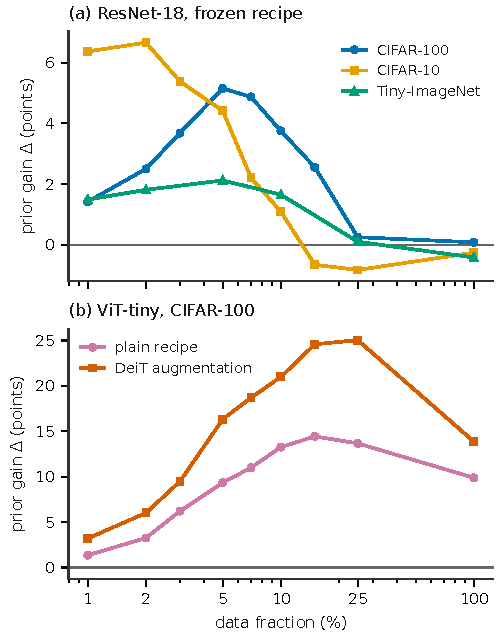
\includegraphics[width=0.78\linewidth]{figs/envelopes.pdf}
\caption{The prior's gain across the data axis. \textbf{(a)} On convolutional
backbones the envelope is unimodal and neutral at sufficiency under the frozen
epoch-based recipe; the peak tracks task difficulty rather than fraction, and
at a matched step budget the right flank does not appear at all (article,
Sec.~\ref{sec:dataopt}). \textbf{(b)} On ViT-tiny the gain is large at \emph{every}
scale, and DeiT-strength augmentation amplifies rather than replaces it.}
\label{fig:envelopes}
\end{figure}

\end{document}
